\section{Patched Dynamical Models}
A variety of methods exist to model the gravitational forces of three (or more) celestial bodies in
dynamical systems. While a high-fidelity ephemeris model (HFEM) provides the best accuracy, some
models utilize simplifying assumptions to reduce computations and gain more insight into the
dynamics of the system while maintaining adequate fidelity. For including all of the bodies in one
model, there exist several 4-body problems that differ in layout, coherency, and fidelity. Some of
the more prominent options are the (BCR4BP)\cite{Boudad:2018}, Hills restricted 4-body problem
(HR4BP)\cite{Scheeres:1998}, and quasi-bicircular restricted 4-body problem
(QBCR4BP)\cite{Andreu:2002}. A different approach, and the one used in this investigation, is to
patch together 2BP and CR3BP models to build a larger model to represent the dynamics. Two such
patched models are outlined here.

\subsection{The Patched 2BP-CR3BP Model}
A patched 2BP-CR3BP model is used to describe trajectories as they move between CR3BP systems via a
2BP system. An example from this investigation is leaving the Sun-Earth CR3BP into heliocentric
space (modeled as a 2BP) before entering the Sun-Mars CR3BP. While the spacecraft is near a planet,
it is modeled in the Sun-planet CR3BP. But once it reaches a specified distance from that planet,
it is modeled instead using Keplearian 2BP motion around the Sun\cite{Canales:2021b}. The interface
location between the two models is called the sphere of influence (SoI) since it represents where
the gravitational influence of the planet becomes negligible compared to that of the Sun.

Trajectories computed in this model are best represented by using a coordinate frame centered on
the focus of the 2BP, the Sun in this example. In this investigation, trajectories in the 2BP-CR3BP
patched model are shown in the Sun-centered Ecliptic J2000 Frame, as described in Section 2.1.2.
Although the Sun-Earth CR3BP is coplanar with this frame, the Sun-Mars CR3BP system is not and Mars
is considered to be located at its respective orbital inclination. The $XY$-projection of an
example 2BP-CR3BP patched model system is shown in \cref{fig:2BP-CR3BP}.

\begin{figure}[H]
    \centering
    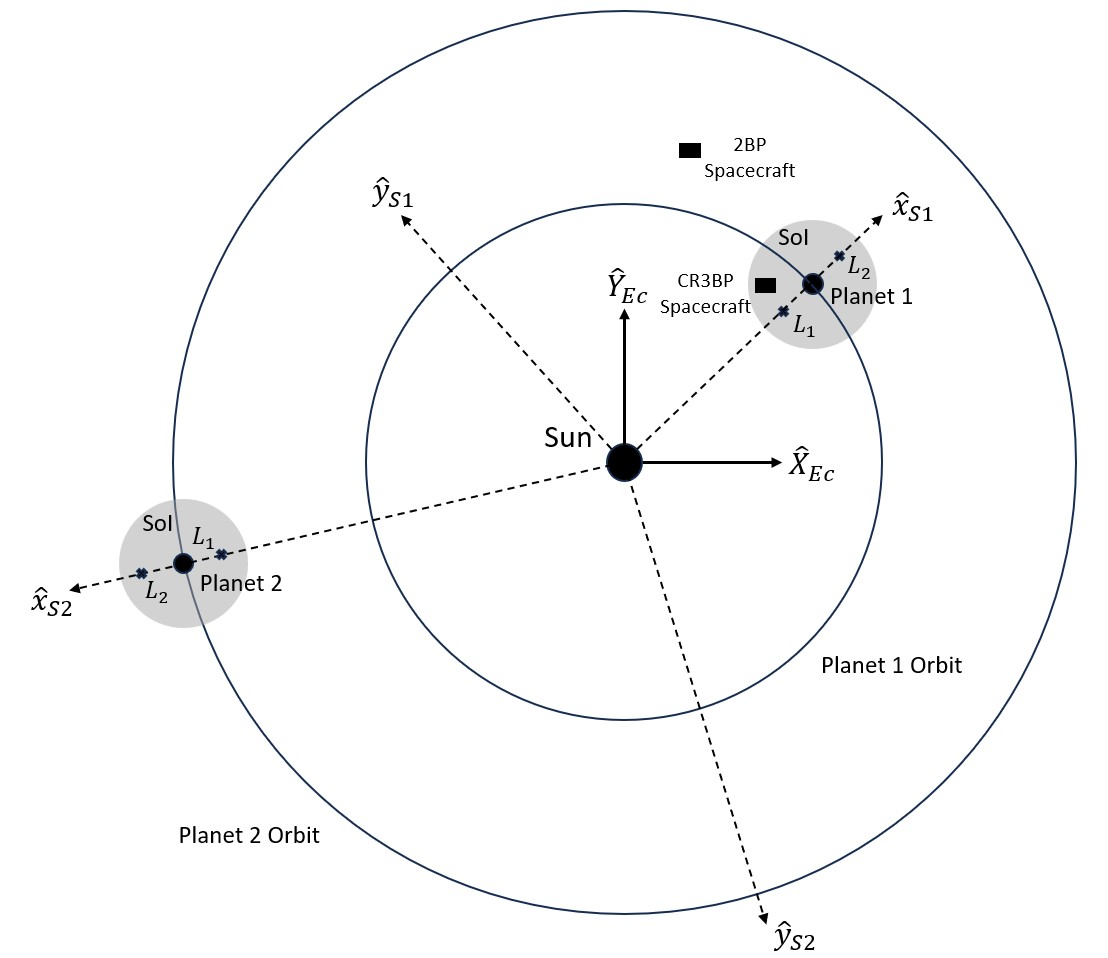
\includegraphics[width=0.75\textwidth]{figures/TBP-CR3BP.jpg}
    \caption{$XY$-Projection of the Patched 2BP-CR3BP Model}
    \label{fig:2BP-CR3BP}
\end{figure}

The radius of the SoI is a design parameter dependent on the application. For this patched model,
an SoI is desired such that CR3BP periodic orbits around the Lagrange points are included,
demonstrated in \cref{fig:SoI}. By defining a gravitational ratio:
\begin{equation}
    d_{SoI}=\frac{g_{2}}{g_{1}},
    \label{eq:patchedSoI}
\end{equation}
where $g_{i}$ is the gravitational acceleration of the respective primary body at a specified
location, an SoI radius from the planet can be chosen so that $d_{SoI}$ is sufficiently small,
i.e., the osculating (instantaneous) orbital elements remain near constant in the
CR3BP\cite{Canales:2021b}.

\begin{figure}[H]
    \centering
    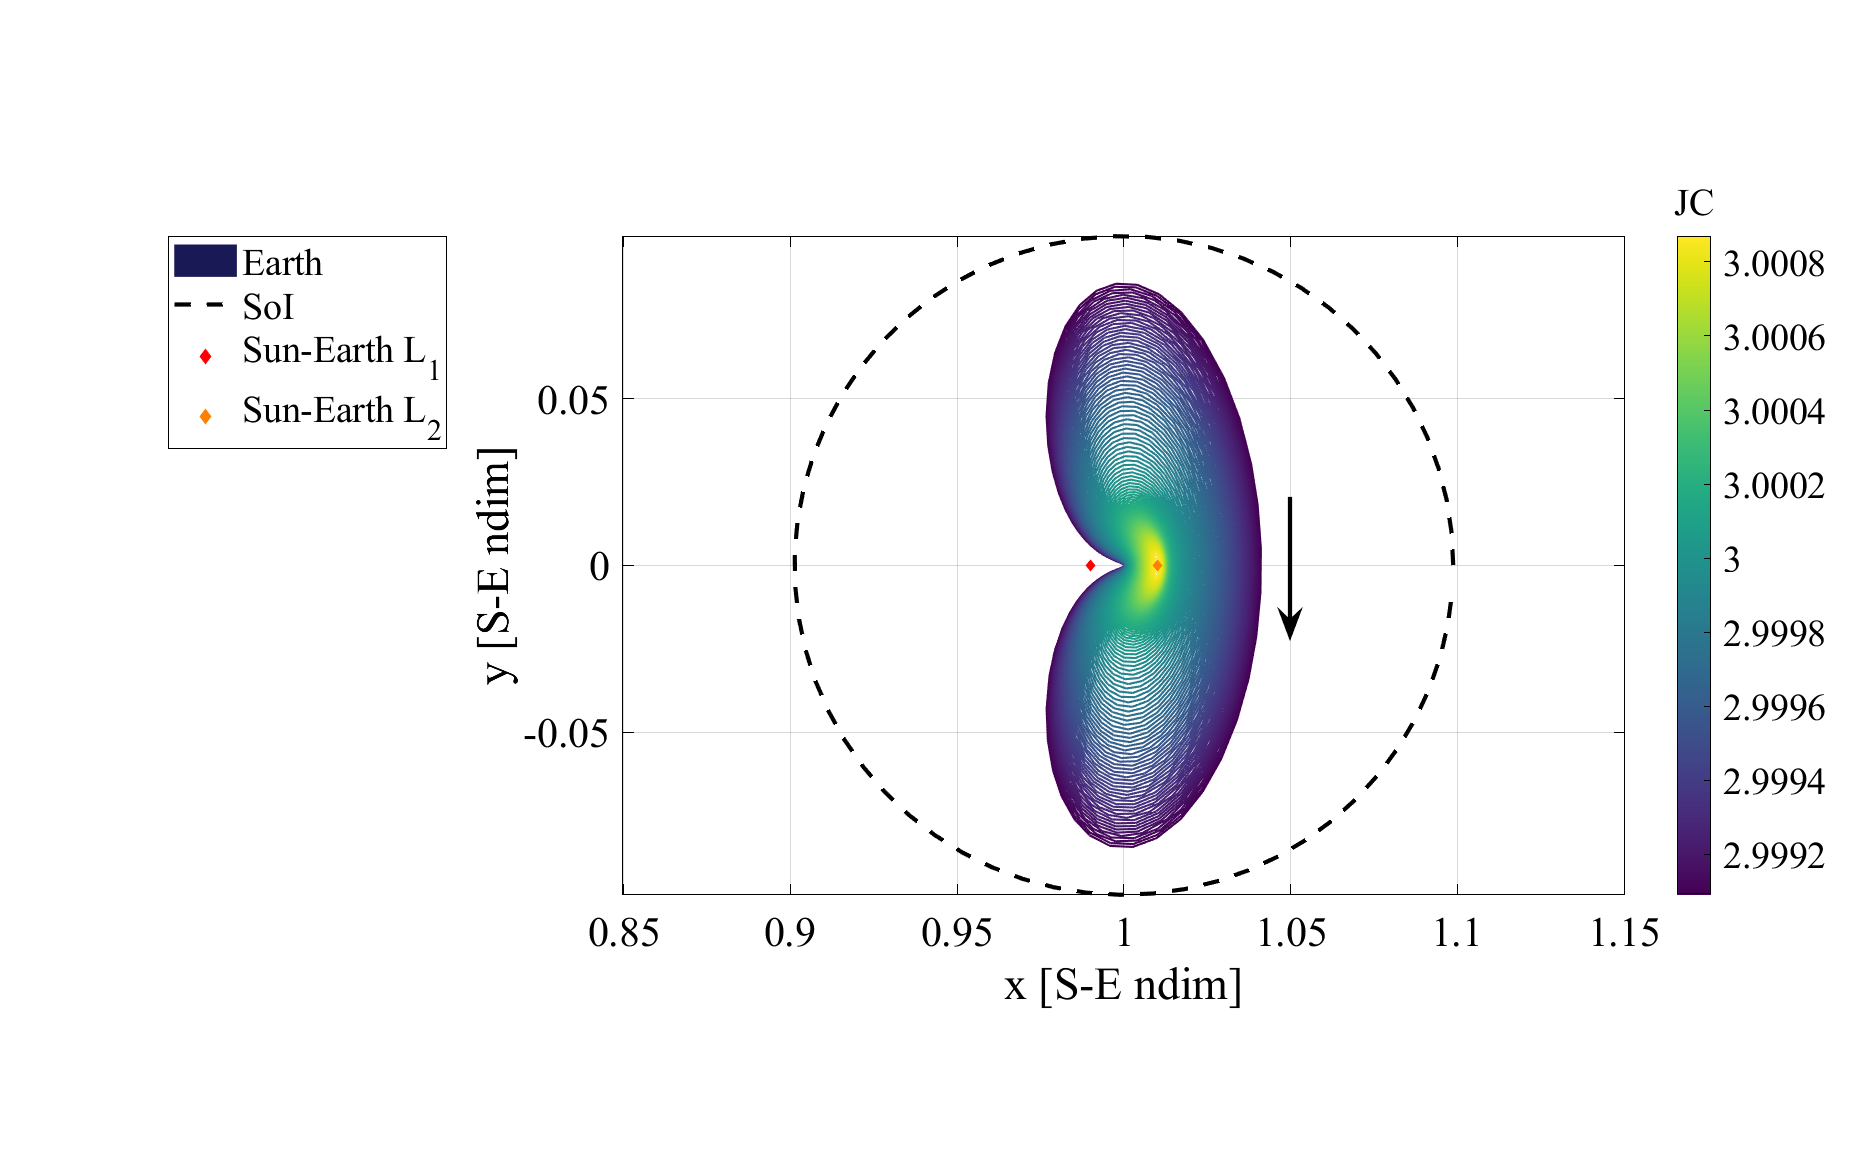
\includegraphics[width=0.9\textwidth]{figures/SoI.pdf}
    \caption{Patched 2BP-CR3BP sphere of influence around Earth, encompassing a large portion of the Sun-Earth $L_{2}$ Lyapunov family.}
    \label{fig:SoI}
\end{figure}

\subsection{The Blended CR3BP Model}
Two CR3BP models can be blended to form a 4-body model if one of the primary bodies is present in
both models. For example, a Sun-Earth CR3BP can be blended with an Earth-Moon CR3BP to form a
Sun-Earth-Moon 4-body problem (here, the Earth is the common primary). This method incorporates the
difference in inclinations between the two CR3BP models but is now a time-dependent
model\cite{Kakoi:2014}. Similar to the patched 2BP-CR3BP model, the boundary between the two models
is at an SoI, now around the smaller primary of the smaller CR3BP model (the Moon in this example).

Unlike the patched model above, this model is best represented in the barycentric rotating frame of
the larger CR3BP model (the Sun-Earth rotating frame in this example). Since the blended model is
time-dependent, the portion of the trajectory computed in the smaller CR3BP will be shifted when
represented in the larger model depending on the epoch. The $xy$-projection of an example blended
system is shown in \cref{fig:BlendedCR3BP}.

\begin{figure}[H]
    \centering
    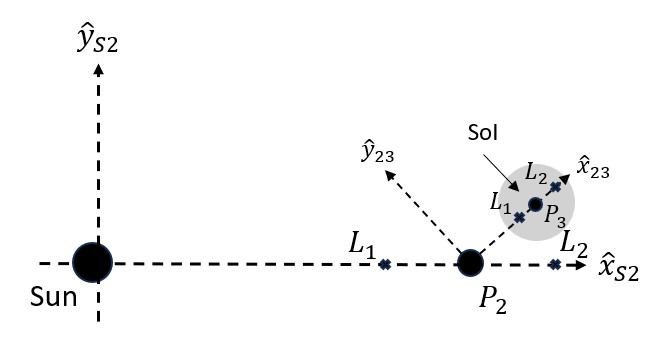
\includegraphics[width=0.5\textwidth]{figures/BlendCR3BP.jpg}
    \caption{$xy$-Projection of the Blended CR3BP Model}
    \label{fig:BlendedCR3BP}
\end{figure}

The SoI radius used for the blended model is different from that used for the patched model. As
mentioned before, this SoI is centered around the second primary of the smaller system and the
gravitational accelerations being compared are the first primary of the larger system and the
smaller primary of the second system (e.g., the Sun and the Moon). A blended CR3BP SoI radius is
defined as:
\begin{equation}
    r_{SoI}=l^{*}_{12}(\frac{m_{3}}{m_{1}})^{2/5},
    \label{eq:blendedSoI}
\end{equation}
where the primaries are numbered in order of decreasing mass\cite{Parker:2013}.
